\section{Spectral Approach}
\label{sec:spectral}

%connected,related
%In this section we show that the spectrum of the transfer operator is highly connected to the metastability of the corresponding Markov process.
In this section, we demonstrate the strong relation of the metastability of a Markov process to the spectrum of the associated transfer operator. %associated/corresponding
%spectrum of the transfer operator to the metastability of the corresponding Markov process.
More precisely, the existence of metastable sets implies the existence of dominant eigenvalues of the transfer operator and vice versa.
The idea to detect metastable sets via dominant eigenvalues has been first proposed by Dellnitz and Junge\cite{dellnitz1999approximation} and transferred to molecular dynamics by Sch\"utte et al\cite{schutte1998conformational,schutte1999direct}.

\subsubsection*{Existence of dominant eigenvalues}

%The \textit{multiplicity} of an eigenvalue $\lambda$ is defined as the dimension of the generalized %eigenspace. Eigenvalues of multiplicity $1$ are called  \textit{simple}.

%Let us, lag-time t
We consider the transfer operator $\Pcal := \Pcal(\tau)$ of a Markov process for some fixed lag-time $\tau$ in the Hilbert space $L^2(\mu)$. \marginpar{ $L^2$, $L^1$?}
%$L^1$ Huisinga diss; why $L^2$, $L^1$ enough?
%For further informations, see Kato\cite{kato1995}.
We are interested in \textit{dominant eigenvalues} of $\Pcal$, that is large eigenvalues which are close to 1 and separated from the rest of the spectrum.
The \textit{discrete spectrum} $\sigma_{\mathrm{discr}}(\Pcal)$ is the set consisting of all eigenvalues $\lambda \in \sigma(\Pcal)$ that are isolated and of finite multiplicity.
%contains all
The \textit{essential spectral radius} $r_{\mathrm{ess}}(\Pcal)$ is defined as
\begin{equation*}
r_{\mathrm{ess}}(\Pcal) = \inf \{ r \geq 0 \mid \lambda \in \sigma(\Pcal) \textrm{ with } |\lambda| > r \textrm{ implies } \lambda \in \sigma_{\mathrm{discr}}(\Pcal) \}.
\end{equation*}
%essential/continuous. under consideration
The existence of dominant eigenvalues requires that the continuous part of the spectrum is bounded away from the dominant elements of the discrete spectrum.
To ensure that the process we are considering actually possesses metastable sets, we need to pose some conditions on the spectrum of the transfer operator:
\begin{description}
    \item[C1] The essential spectral radius of $\Pcal$ is less than one, i.e. $r_{\mathrm{ess}} < 1$.
    \item[C2] The eigenvalue $\lambda=1$ of $\Pcal$ is simple and dominant, i.e.
    %i.e. $\eta \in \sigma(\Pcal)$ with $|\eta| = 1$ implies $\eta = 1$.
    \begin{equation*}
    \eta \in \sigma(\Pcal) \textrm{ with } |\eta| = 1 \textrm{ implies } \eta = 1.
    \end{equation*}
\end{description}
%criteria for it
We will not go into further details for which processes the two above conditions are fulfilled; some criteria can be found in Huisinga\cite[chapter $4$]{huisinga2001metastability}.
Since we are interested in a metastable behaviour, we assume that the processes under investigation satisfy these conditions.
%Since these conditions are required for the later investigations, we will just assume that they are true.
We need condition {\textbf{\textsf{C1}} to ensure that the continuous part of the spectrum is bounded away from the discrete eigenvalues. Otherwise they would not be dominant anymore and the process would be rather rapidly mixing than having any metastable sets.
%metastable sets/dominant structures
Condition {\textbf{\textsf{C2}} however is important because the state space of a transfer operator with more than one eigenvalue of absolute value $1$ can be decomposed into invariant sets, that is subsets which cannot be left. \marginpar{absolute?}
%\marginpar{C2 = ergodic?}
%\marginpar{has periodic structures?}
%stable/invariant
However, such a case is not interesting for us.
%\marginpar{excludes modeling and interpretation problems}
Instead, we want to know more about \textbf{almost} invariant sets and their critical transition regions. 
%We will consider only ergodic process which means theat the eigenvalue $1$ is unique.
\\


%transfer operator for a process unique?
The transfer operator $\Pcal: L^2(\mu) \rightarrow L^2(\mu)$ of a reversible process satisfying the properties \textrm{\textbf{\textsf{C1}}} and \textrm{\textbf{\textsf{C2}}} is self-adjoint by theorem \ref{thm:selfadjoint_reversible} and has a spectrum of the form
%has a spectrum of the form/the following spectrum
%\marginpar{why discr. rechts?}
\begin{equation*}
\sigma(\Pcal) \subset [a,b] \cup \{\lambda_n\} \cup \dots \cup \{\lambda_2 \} \cup \{1\}
\end{equation*}
with $-1 < a \leq b < \lambda_n \leq \dots < \lambda_1 = 1$ and isolated, not necessarily simple eigenvalues of finite multiplicity that are counted according to multiplicity.


\subsubsection*{Relation of dominant spectrum to metastability}

%state,determine
In order to find out about the quality of an arbitrary decomposition, we present upper and lower bounds for the metastability of the decomposition in terms of dominant eigenvalues and eigenvectors of the transfer operator.
We will denote by \textit{metastability of a decomposition $\Dcal$} the sum of the metastability of its subsets.

%Sch\"utte\cite[theorem 4.16]{schutte2013metastability}
\begin{thm}[{Huisinga and Schmidt\cite[Theorem 2.4]{huisinga2006metastability}}]
\label{thm:metastability_bounds_1}
Let $\Pcal$ be the transfer operator of a reversible process satisfying \textrm{\textbf{\textsf{C1}}} and \textrm{\textbf{\textsf{C2}}}.
Let $\lambda_1,\dots,\lambda_n$ denote its isolated eigenvalues and $v_1,\dots,v_n$ the corresponding eigenfunctions, normalized to $\Vert v_i \Vert_2 = 1$.
Let $Q$ be the orthogonal projection of $L^2(\mu)$ onto $\mathrm{span}\{\eins_{A_1},\dots, \eins_{A_n}\}$.
The metastability of an arbitrary decomposition $\Dcal = \{A_1,\dots, A_n\}$ of the state space $E$ can be bounded from above by
\begin{equation*}
p(A_1,A_1) + \dots + p(A_n, A_n) \leq 1+ \lambda_2 + \dots + \lambda_n,
\end{equation*}
while it is bounded from below by
\begin{equation*}
1+ \rho_2 \lambda_2 + \dots + \rho_n \lambda_n + c \leq p(A_1,A_1) + \dots + p(A_n, A_n),
\end{equation*}
where $\rho_j = \Vert Q v_j \Vert_{L^2(\mu)}^2 = \langle Qv_j, Qv_j \rangle \in [0,1]$ and $c = a(1-\rho_1) \cdots (1 - \rho_n)$.
\end{thm}

%shows,reveals. relation/connection. eigenfunctions and eigenvalues
Theorem \ref{thm:metastability_bounds_1} reveals the strong relation between metastable sets and the dominant eigenvalues of the transfer operator.
%enables,allows,provides us an insight into. evaluate,judge,rate
It allows us to evaluate the quality of a decomposition by comparing the lower and the upper bound of metastability.
The upper bound shows that eigenvalues far away from $1$ worsen the metastability of a decomposition.
The lower bound is close to the upper bound if the dominant eigenfunctions $v_2,\dots,v_n$ are almost constant on the metastable subsets $A_1,\dots,A_n$, implying $\rho_j \approx 1$ and $c \approx 0$.
Moreover, Huisinga and Schmidt\cite{huisinga2006metastability} show that the lower and upper bounds from theorem \ref{thm:metastability_bounds_1} are sharp and asymptotically exact.

That provokes the question if there exists an \textbf{optimal} decomposition with the highest possible metastability. \marginpar{maybe ill-conditioned}
%In fact, this problem might unfortunately be ill-conditioned.
By all means, this theorem indicates that the number of metastable sets should be determined by the number of dominant eigenvalues.
\\

Deuflhard et al\cite{deuflhard2000identification} proposed an algorithm to identify the metastable sets of a Markov chain by exploiting the sign structure of the dominant eigenvectors of the transition matrix.
\\

In figure \ref{fig:spectrum}, we get a good overview of the relation between the eigenfunctions of the transfer operator and the metastable sets of the corresponding process. We have a potential/energy landscape with 4 energy minima, that is 4 regions where the process could be \textit{trapped} such that it is hard to get outside again. The transition matrix  shows this metastable behaviour since we can see 4 regions which large probabilities to stay inside and very small probabilities to go to a different region.
Furthermore we see that the process has 4 dominant eigenvalues. Three of them have a change of sign, inducing a metastable decomposition.
\newpage


\begin{figure}[!ht]
	\label{fig:spectrum}
	\centering
	\subfigure[Transition matrix $P$ on $100$ states with $4$ visible metastable sets]{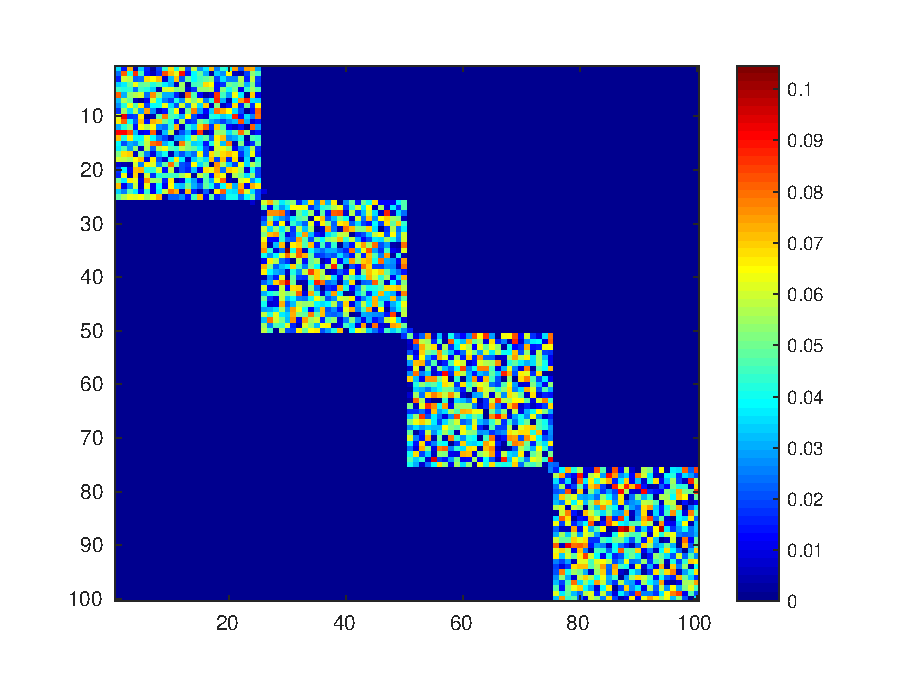
\includegraphics[width=0.49\textwidth]{figures/spectral/transition.eps}}
	\subfigure[Spectrum of $P$ with $4$ dominant eigenvalues]{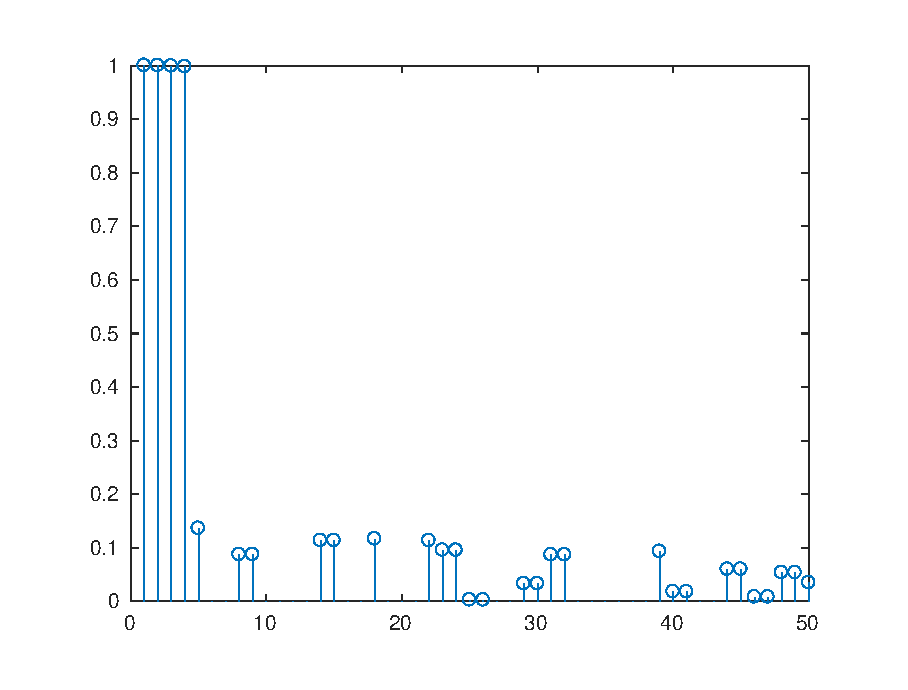
\includegraphics[width=0.49\textwidth]{figures/spectral/eigenvalues.eps}}
	\subfigure[Dominant eigenvectors of $P$ with change of signs corresponding to the transition regions]{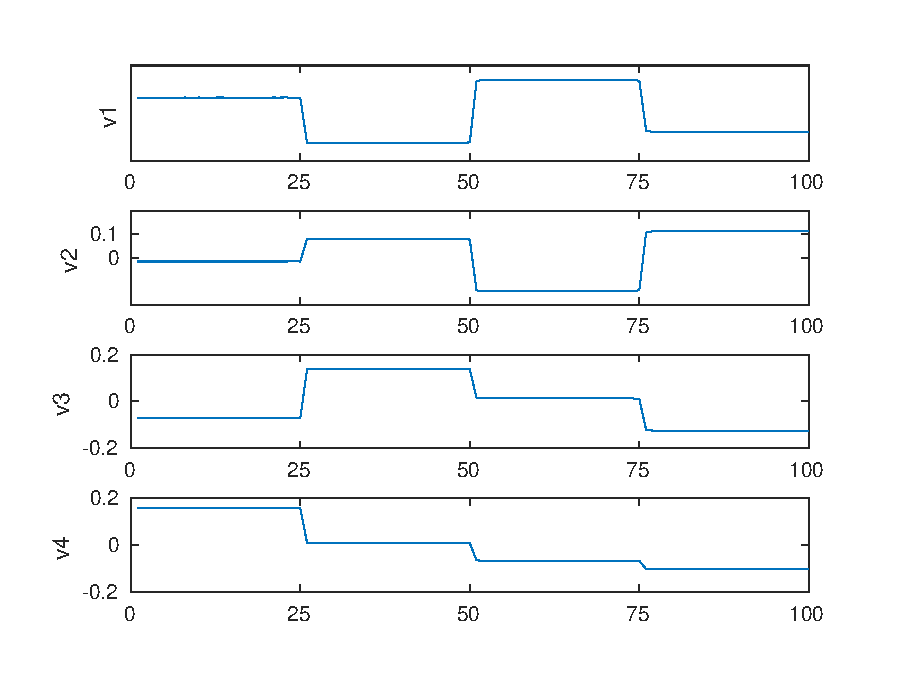
\includegraphics[width=0.49\textwidth]{figures/spectral/eigenvectors.eps}}
	\caption{Relation of the transition matrix to its spectrum with regard to metastability}
\end{figure}

%anschaulich
%This theorem gives us a first demonstrative relation of the metastability of a process to its eigenvectors. This %result is not yet optimal/very good. In the next sections, we will see that linear combinations of eigenvectors %result in much better metastability.


This relation can be explained as follows.
A process consisting of $n$ invariant sets $\{A_1,\dots,A_n\}$ has the $n$-fold eigenvalue $1$ and the corresponding eigenvectors $\eins_{A_i}$ are constant on the invariant sets.
A metastable process consists of almost invariant sets and thus, can be interpreted as the perturbation of a process with invariant sets, by introducing small transitions between the invariant sets. Accordingly, the eigenvalues and eigenvectors are perturbed. This results in one eigenvalue $1$ and $n-1$ eigenvalues close to $1$, having eigenvectors that are almost constant on the almost invariant sets.
A detailed perturbation analysis can be found in Deuflhard et al\cite{deuflhard2000identification}.

\subsubsection*{Disadvantages}
%Conclusion
%Advantages, Alternatives

%suitable,convenient
%to characterize metastability of Markov processes, respectively. wrt its metastable sets
%convenient,suitable,possible,feasible
The spectral approach is an appropriate method to cluster a process with respect to metastability, though it bears some disadvantages.
%1:
The result is only appliable on reversible processes, because real eigenvalues are only guaranteed if the transfer operator is self-adjoint. \marginpar{see}
%2:
%Moreover, the eigenvector problem of the transfer operator has only global solutions. \marginpar{global = good?}
%Most of all,
Particularly, the previous procedure to compute a metastable decomposition does not take into consideration the existence of transition regions.
This can lead to an iteration error, i.e. the clustered process does not represent the correct long-time behaviour.
%needs refinement/improvement
\\

%clarify/point out/emphasize/highlight
This section has been presented mainly with the aim to emphasize the strong relation of the spectrum of the transfer operator to the metastability of the system. %mainly/merely/solely/only
%results in a full partition decomposition and
However, this approach does \textbf{not} represent the state of the art.
%This relation can be seen best for a full partition decomposition/clustering.
%enhanced/improved. related, but improved,
In the next section, we deduce an enhanced method, resulting in a \textbf{soft} clustering instead of a full partition decomposition.
%, which likewise takes advantage of this strong relation between spectrum and metastability.
%It also includes the eigenvalues and eigenfunctions of the transfer operator, but will be soft instead of crisp.
%comprises/includes the eigenvalues and eigenfunctions of the transfer operator, but it will be fuzzy.
